\documentclass[a4paper]{article}
\usepackage{titlesec}
\setcounter{secnumdepth}{4}

\titleformat{\paragraph}
{\normalfont\normalsize\bfseries}{\theparagraph}{1em}{}
\titlespacing*{\paragraph}
{0pt}{3.25ex plus 1ex minus .2ex}{1.5ex plus .2ex}




\usepackage{graphicx}
\usepackage[portuguese]{babel}
\usepackage[utf8]{inputenc}
%opening
	\title{Análise do Sistema \\ Letrinhas \\ APP \& Sistema de Informação }
\author{Projecto de Sistemas de Informação}



\begin{document}

	\maketitle %titulo
  
	\newpage
	\tableofcontents %indice
	\newpage %pagina nova

	 \section{Introdução}%resumo - introdução
		\subsection{Visão Geral do Sistema}
		 
		A questão apresentada ao grupo de trabalho consiste na criação de um sistema que permita a avaliação de alunos do ensino básico, em diversas áreas, nomeadamente fluência na leitura, quer ao nível de palavras, quer de textos completos, entre outros tipo de testes como por exemplo interpretação de sons e/ou imagens, sempre através do recurso a um tablet.\\ 

		O sistema será composto por uma aplicação para dispositivos móveis e o respetivo sistema de informação.

		\subsubsection{Aplicação para tablet}
		A aplicação deverá permitir dois tipos de acessos, o do Professor, para fazer a correção dos testes na própria aplicação e o do aluno que através do interface do tablet deverá realizar os testes propostos pelo professor.
		
		\subsubsection{Sistema de Informação}
		O sistema de informação dá suporte à aplicação, recorrendo a uma base de dados e formulários web.

		\subsection{Objetivos}
		
		O Letrinhas tem como principal objetivo permitir a avaliação dos alunos de uma forma simplificada e com diferentes tipos de registos dessa mesma avaliação.\\
		O aluno através do dispositivo móvel terá acesso aos diferentes tipos de testes que serão submetidos previamente pelo professor e avaliados ou no momento ou posteriormente por este. \\
		O sistema de informação estará acessível ao professor e permitirá não só a introdução dos testes, como a revisão de testes efetuados pelos alunos.  


		
		\subsection{Cliente}
		O cliente é o Agrupamento de Escolas Artur Gonçalves, que através  dos docentes da Cadeira de Projetos de Sistemas de Informação, professor António Manso e professor Pedro Dias fizeram a articulação entre as duas partes.
		
		\newpage
		
		\subsection{Fontes e Material de Referência}
		Para melhor compreensão do conceito, utilizamos como material de referência os seguintes.
		
		\subsubsection{Aplicações para gravação de voz}
		\begin{itemize}
			\item eRecorder (Aplicação para android);
			\item Smart Voice Recorder (Aplicação para Android);
			\item Voice Recorder Pro. (Aplicação para Android);
		\end{itemize}
		
		\subsubsection{Aplicações de tradução(Voz para texto)}
		\begin{itemize}
			\item	ListNote Fala-para-texto Notas (Aplicação para Android);
			\item 	Speach to text (Aplicação para Android);
			\item 	Text to speach - Voice to text (Aplicação para Android);
		\end{itemize}
		
		\subsubsection{Software open source}
		\begin{itemize}
			\item	Mi sound recorder (Aplicação para Android);
			\item	Auphonic Software (Aplicação para Android \& Iphone);
			\item	Android Voice Recognition Tutorial;
			\item 	Rehearsal Assistant (Aplicação para Android);
		\end{itemize}
		
		\subsection{Glossário}
			\begin{tabular}{|l|p{10cm}|}
				\hline Android & Sistema operativo para dispositivos móveis. \\ 
				\hline Open Source & Software Informático que respeita as quatro liberdades definidas pela Free Software Foundation. \\  	
				\hline 
			\end{tabular} 
		
		\newpage %pagina nova
		\section{Modelo de Casos de Utilização}
			\subsection{Atores}
		
			\subsubsection{Aplicação}
				\begin{tabular}{|c|p{10cm}|}
					\hline Ator & Descrição \\ 
					\hline Aluno & Ator do sistema que interage diretamente com a aplicação realizando os testes propostos. \\ 
					\hline Professor & Quem distribui e supervisiona o teste realizado pelo aluno. \\ 
					\hline 
				\end{tabular} 
		
			\subsubsection{Sistema de Informação}	
				\begin{tabular}{|c|p{10cm}|}
					\hline Ator & Descrição \\ 
					\hline Administrador & Ator responsável por criar contas de professor, adicionar escolas e alunos ao sistema. \\ 
					\hline Professor & Ator responsável por manipular o conteúdo da base de dados, criar, corrigir e consultar testes de avaliação. \\ 
					\hline 
				\end{tabular} 				
	
	
			
			
			\subsection{Visão geral}
		O sistema irá implementar as funções acima descritas e outras que são efectuadas automaticamente pelo sistema e como tal não são visíveis nos casos de utilização.\\
		
		Aos recolhidos em levantamento de requisitos foram adicionados certos casos de utilização considerados pertinentes.\\
		
		Abaixo temos os diagramas de casos de utilização para uma melhor  visão e compreensão do sistema.

			
			\newpage
			
			\subsection{Diagramas de Casos de Utilização}
			\subsubsection{Casos de utilização da aplicação}
			
			\paragraph{Diagrama de CaU do ator professor e aluno}
			
			\begin{figure}[h]
				\centering
				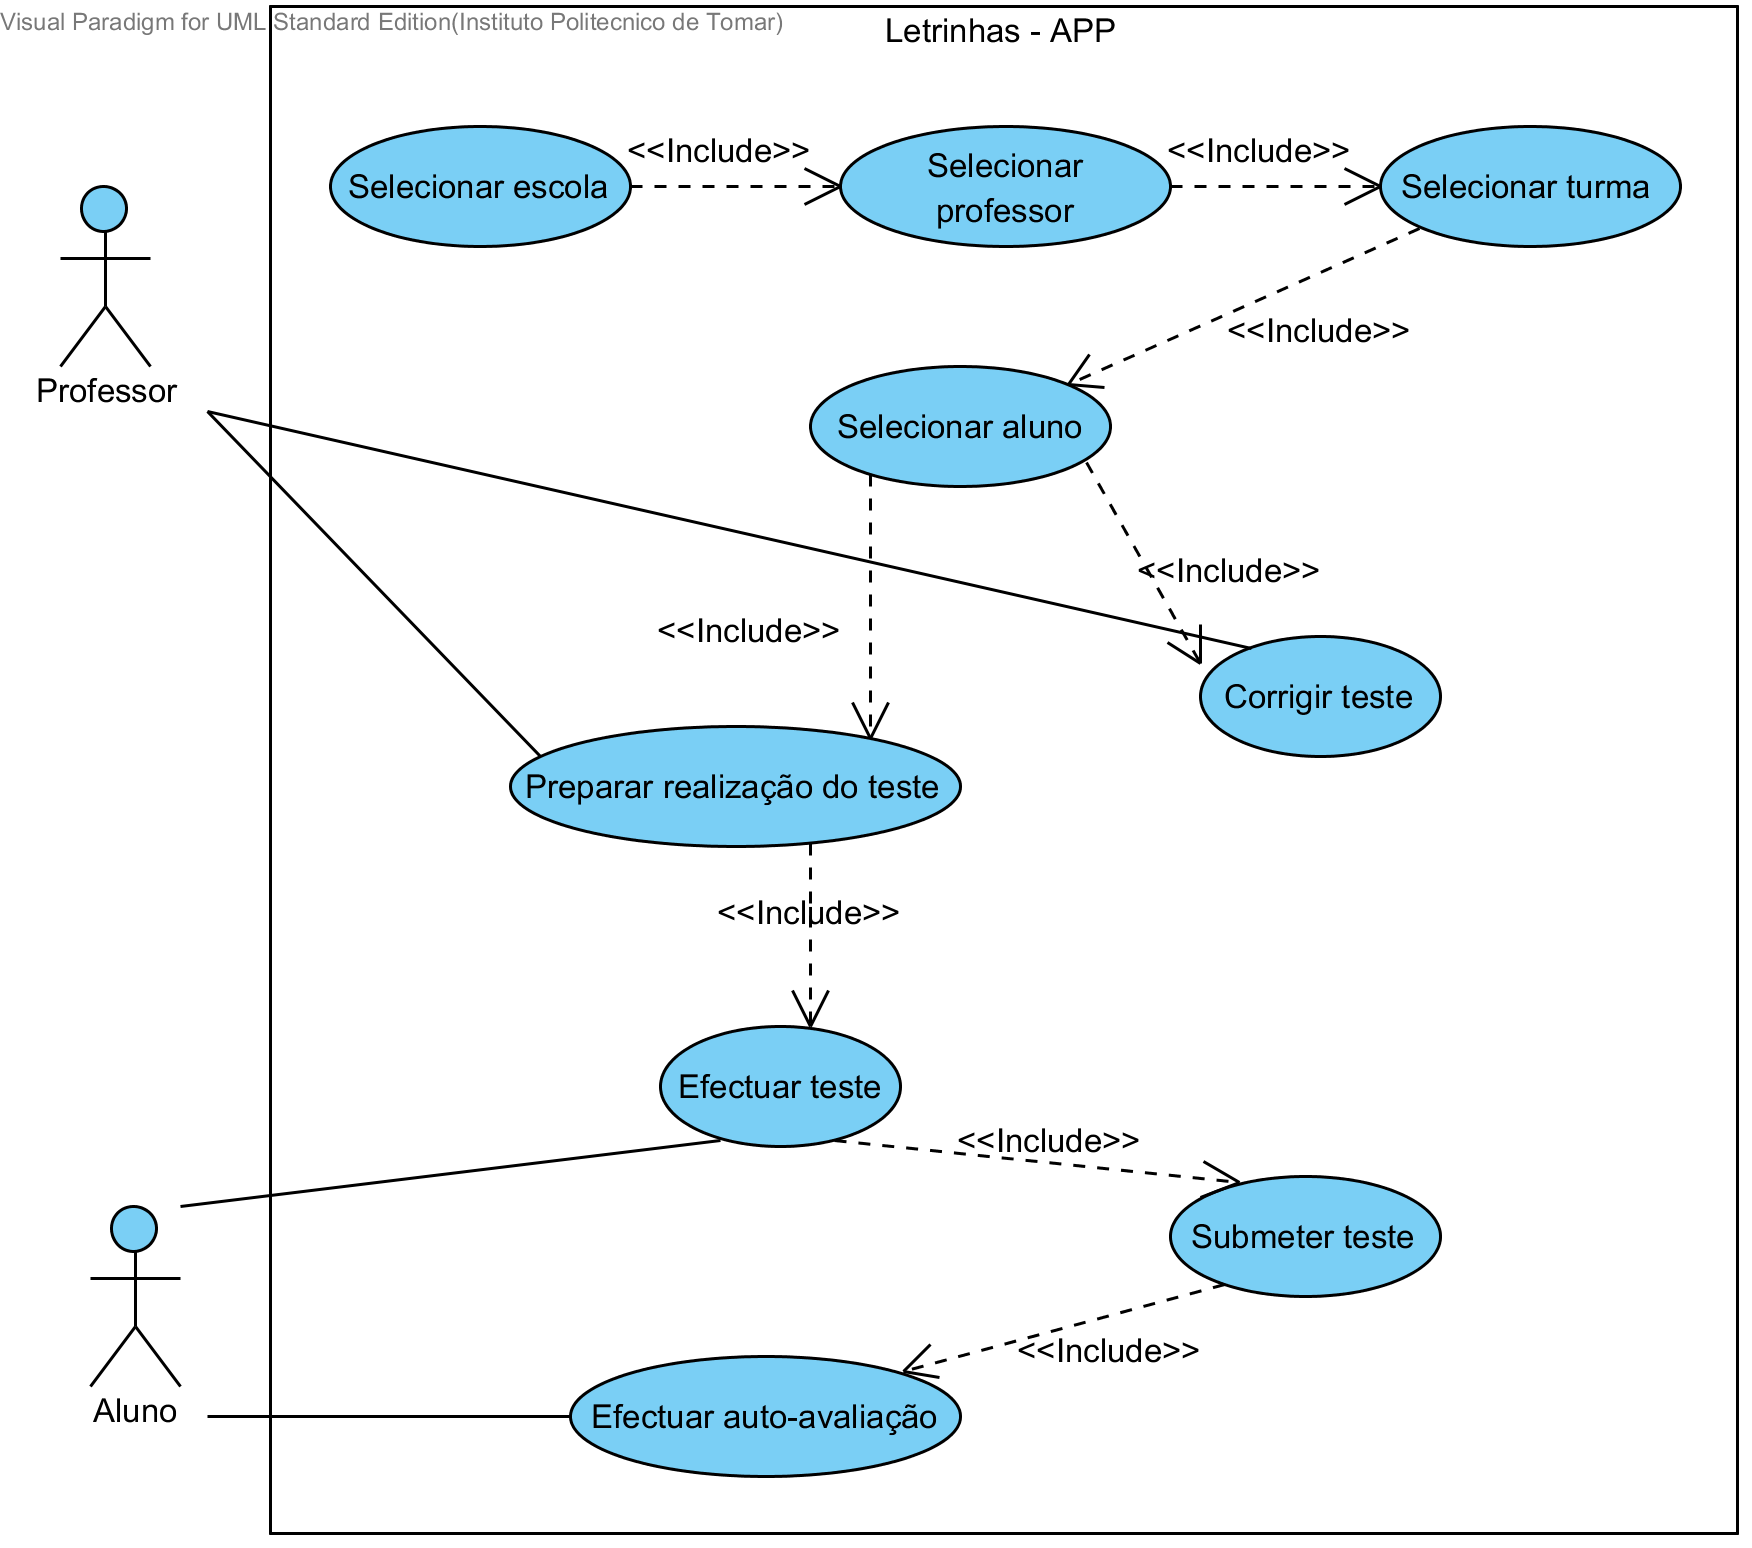
\includegraphics[width=0.8\linewidth]{./diagramasAnaliseSistemas/APP}
				\caption{Casos de Utilização do ator professor e aluno.}
				\label{fig:APP}
			\end{figure}

			Através do diagrama representado na figura 1 podemos observar os casos de utilização do ator professor:
			\begin{itemize}
			\item	Preparar a realização do teste;
			\item   Corrigir teste;
			\end{itemize}
			
			Através do diagrama representado na figura 1 podemos também observar os casos de utilização do ator aluno:
			\begin{itemize}
				\item	Efectuar teste;
				\item   Efectuar Auto-avaliação;
			\end{itemize}
			\newpage
			\subsubsection{Casos de utilização do Sistema de Informação}
						
			\paragraph{Diagrama de CaU do ator administrador e professor}
			
			\begin{figure}[h]
				\centering
				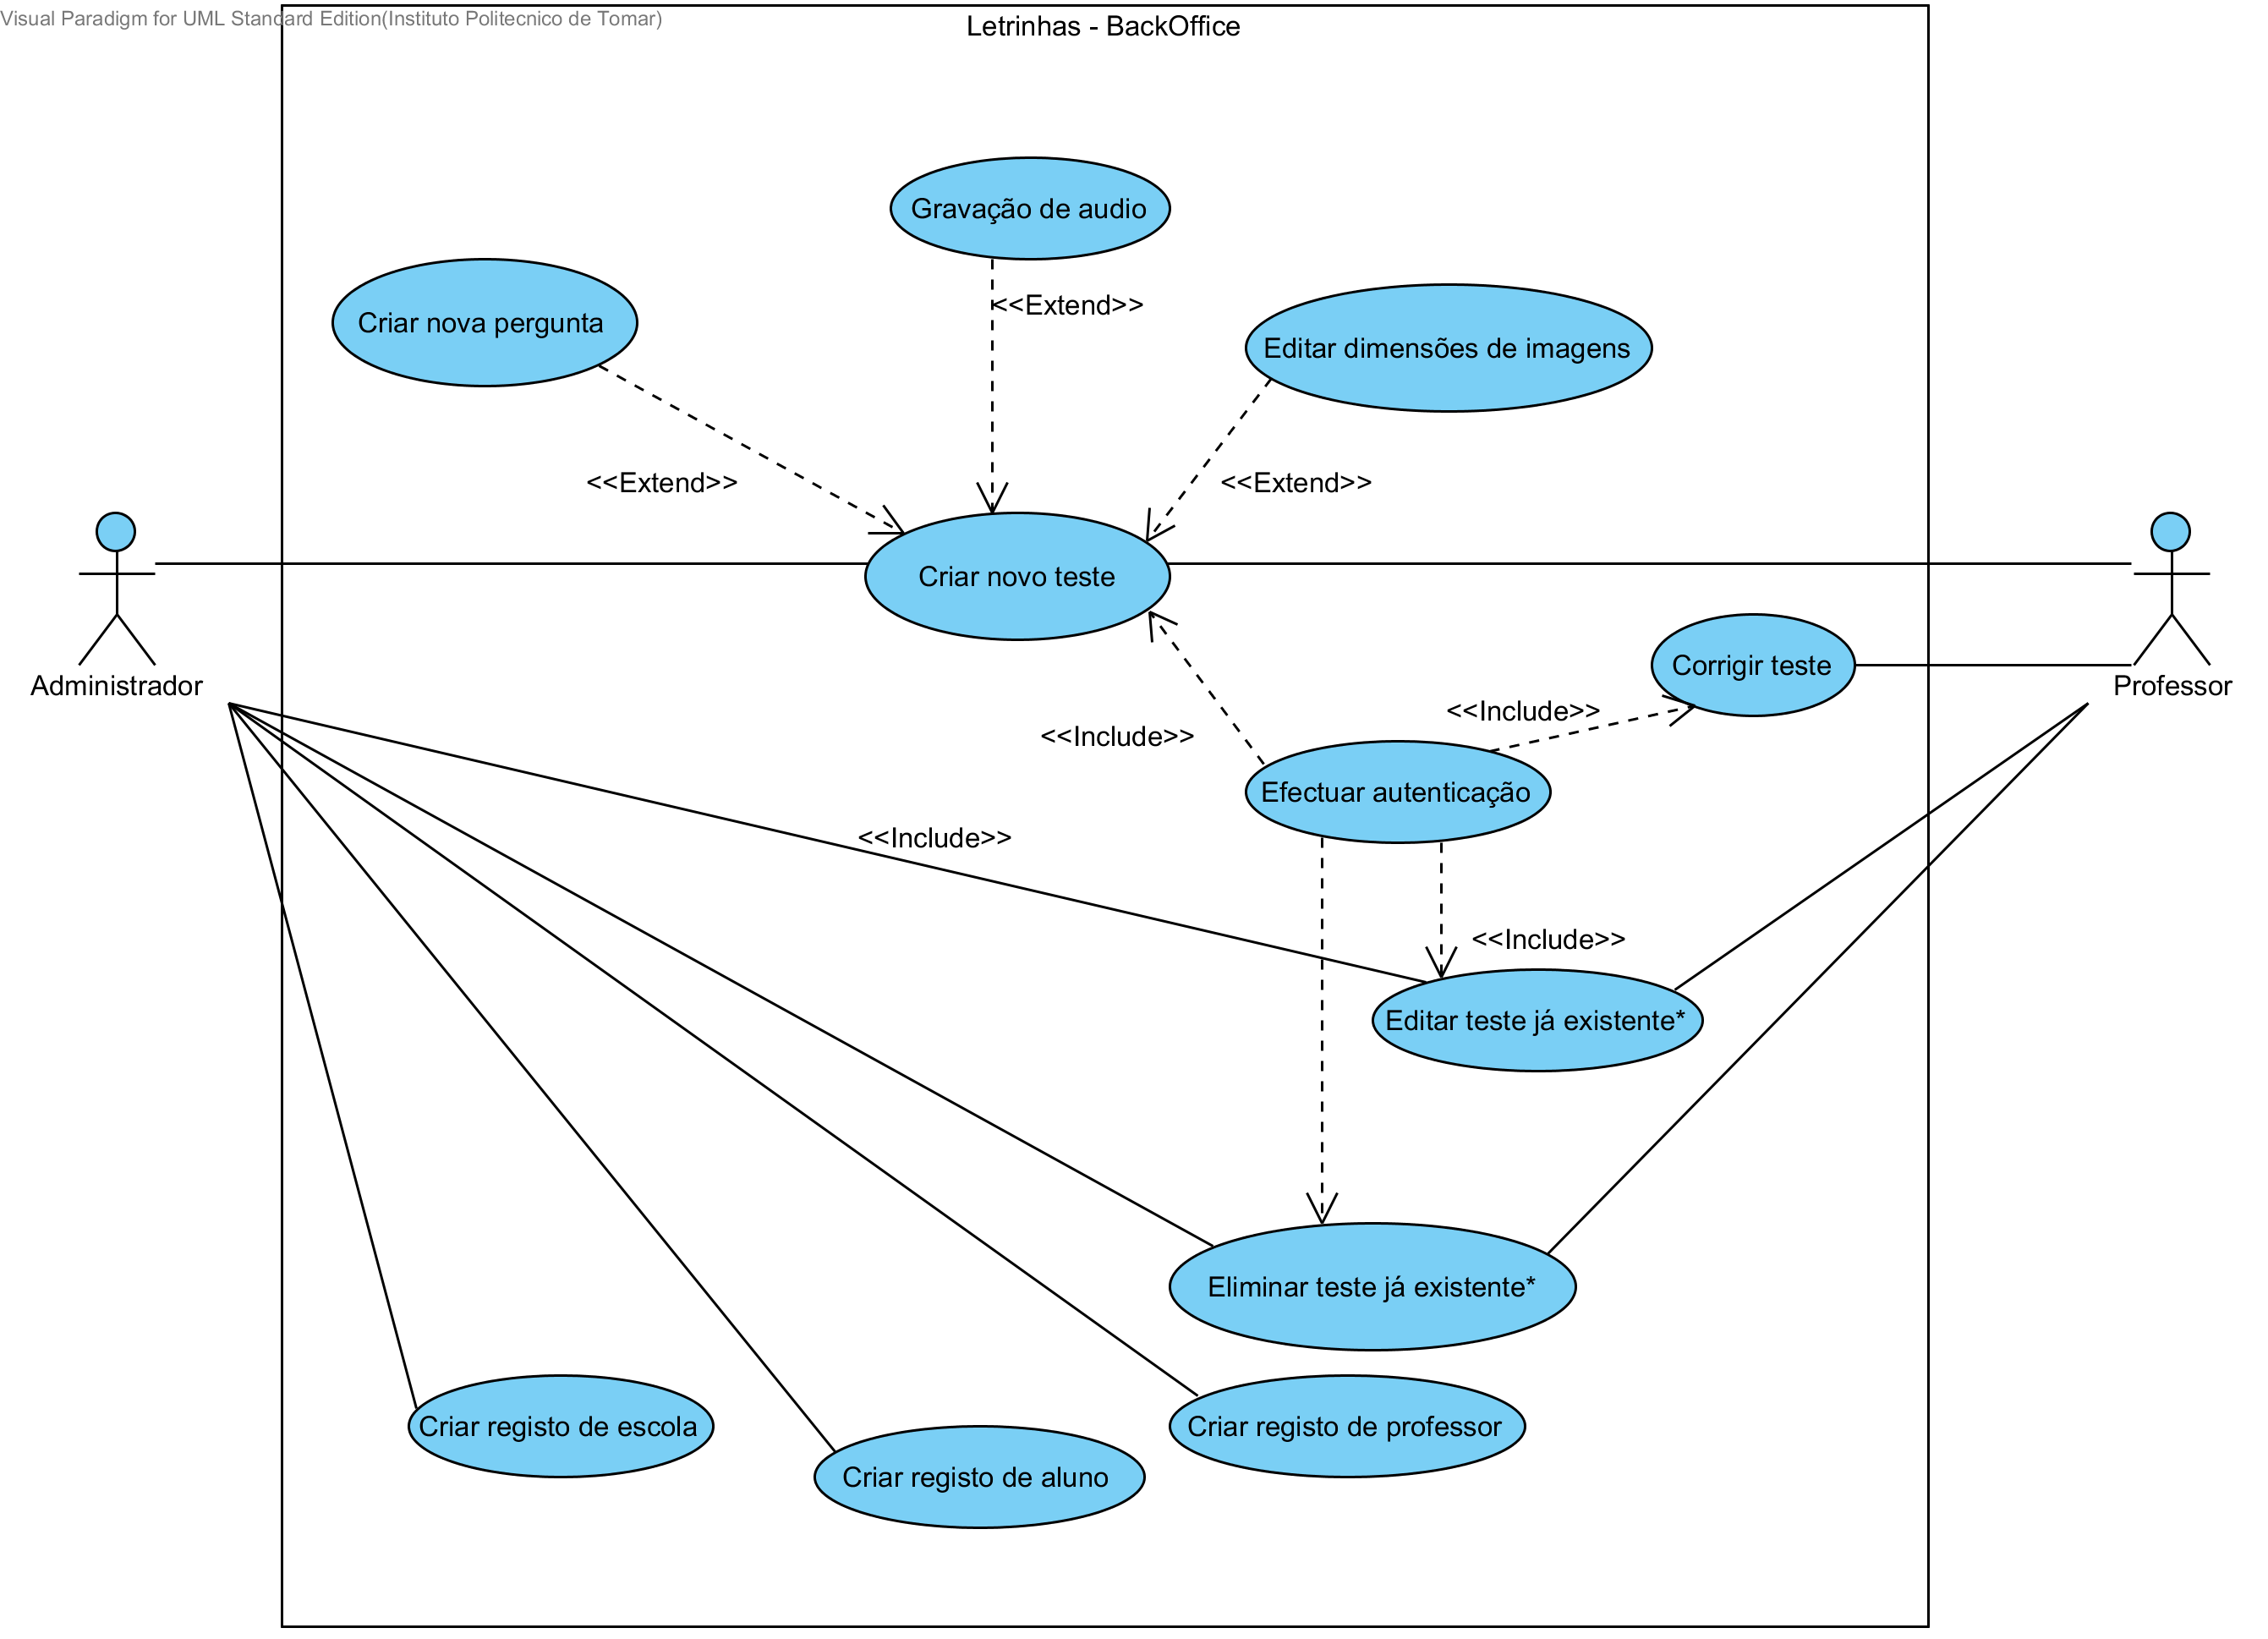
\includegraphics[width=0.8\linewidth]{./diagramasAnaliseSistemas/BackOffice}
				\caption{Casos de Utilização do ator professor e administrador.}
				\label{fig:BackOffice}
			\end{figure}
			Através do diagrama representado na figura 1 podemos observar os casos de utilização do ator adminstrador:
			\begin{itemize}
			\item	Criar novo teste;
			\item   Editar teste já existente;
			\item   Criar registo de professor;
			\item   Criar registo de aluno;
			\item 	Eliminar teste já existente;
			\item   Criar registo de escola;
			\end{itemize}
			
			Através do diagrama representado na figura 1 podemos também observar os casos de utilização do ator professor:
			\begin{itemize}
				\item	Criar novo teste;
				\item   Corrigir teste;
				\item 	Editar teste já existente;
				\item 	Eliminar teste já existente;
				\item   Efectuar Auto-avaliação;
			\end{itemize}
			
			\newpage
			
			\subsection{Descrição dos Casos de Utilização - APP}
					\subsubsection{Corrigir teste}
					\begin{figure}[h]
						\centering
						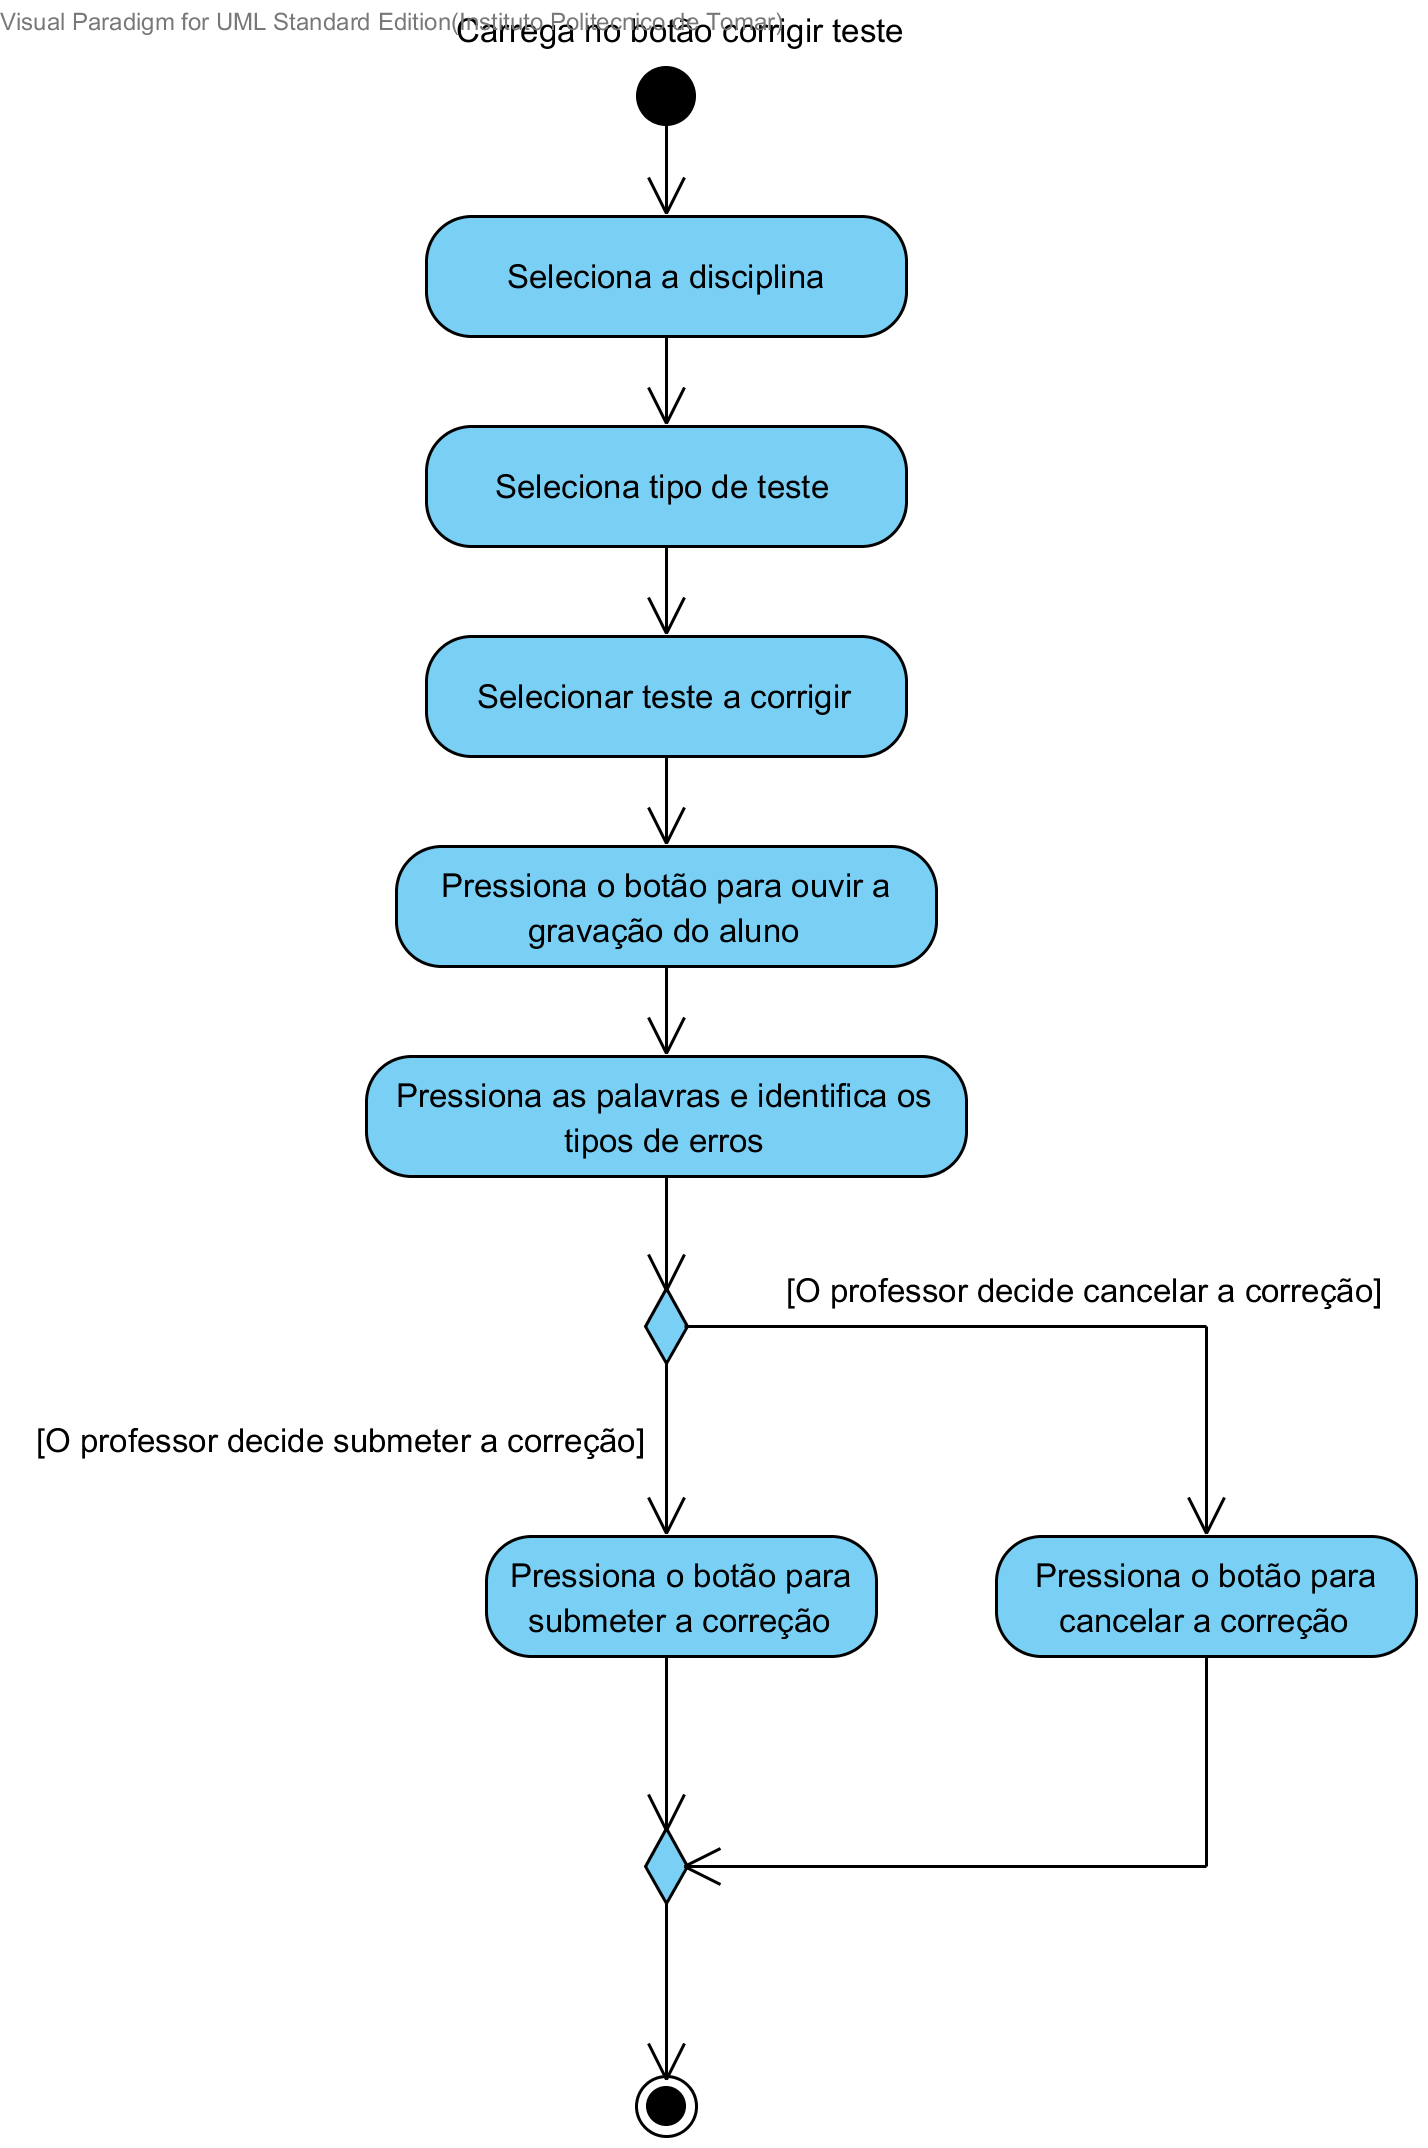
\includegraphics[width=0.7\linewidth]{./diagramasAnaliseSistemas/CorrigirTeste}
						\caption{Diagrama de actividades do C.U. corrigir teste.}
						\label{fig:CorrigirTeste}
					\end{figure}

				\newpage
				\begin {table}[h]
				\begin{tabular}{|p{2cm} p{10cm}|}
					\hline Nome: & CaU Corrigir Teste \\ 
					\hline Âmbito: & Letrinhas - APP \\ 
					\hline Finalidade: & Correcção do teste. \\ 
					\hline Atores: & Professor \\ 
				    \hline Pré-condições: & Deverão existir testes submetidos pelo  aluno.
					O utilizador deverá escolher a  Escola, escolher o professor, escolher a turma, seleccionar o aluno. \\ 
				    \hline Sequência típica dos eventos: &  					
					O utilizador deve:
				    \begin{enumerate}
				    	\item	Seleccionar Corrigir Teste;
						\item	Seleccionar Disciplina;
						\item	Seleccionar o tipo de teste;
						\item	Selecciona o teste a corrigir entre os realizados;
						\item	Ouve a gravação do aluno;
						\item	Corrige;
						\item	Valida a correcção.
				    \end{enumerate} \\ 
  				    \hline Sequências alternativas e extensões: & 
  				    \begin{enumerate}			    	
  				    	\item[4a.] O utilizador cancela a correcção do teste.
  				    \end{enumerate}
  				     \\ 
  				    \hline Requisitos especiais: & Nenhum.\\ 
  				    \hline Aspectos em aberto: & Nenhum. \\
					\hline 
				\end{tabular}
				\caption{Caso de utilização corrigir teste.}
			\end{table} 
			
		\newpage
				\subsubsection{Preparar realização do teste para o aluno}
					\begin{figure}[h]
						\centering
						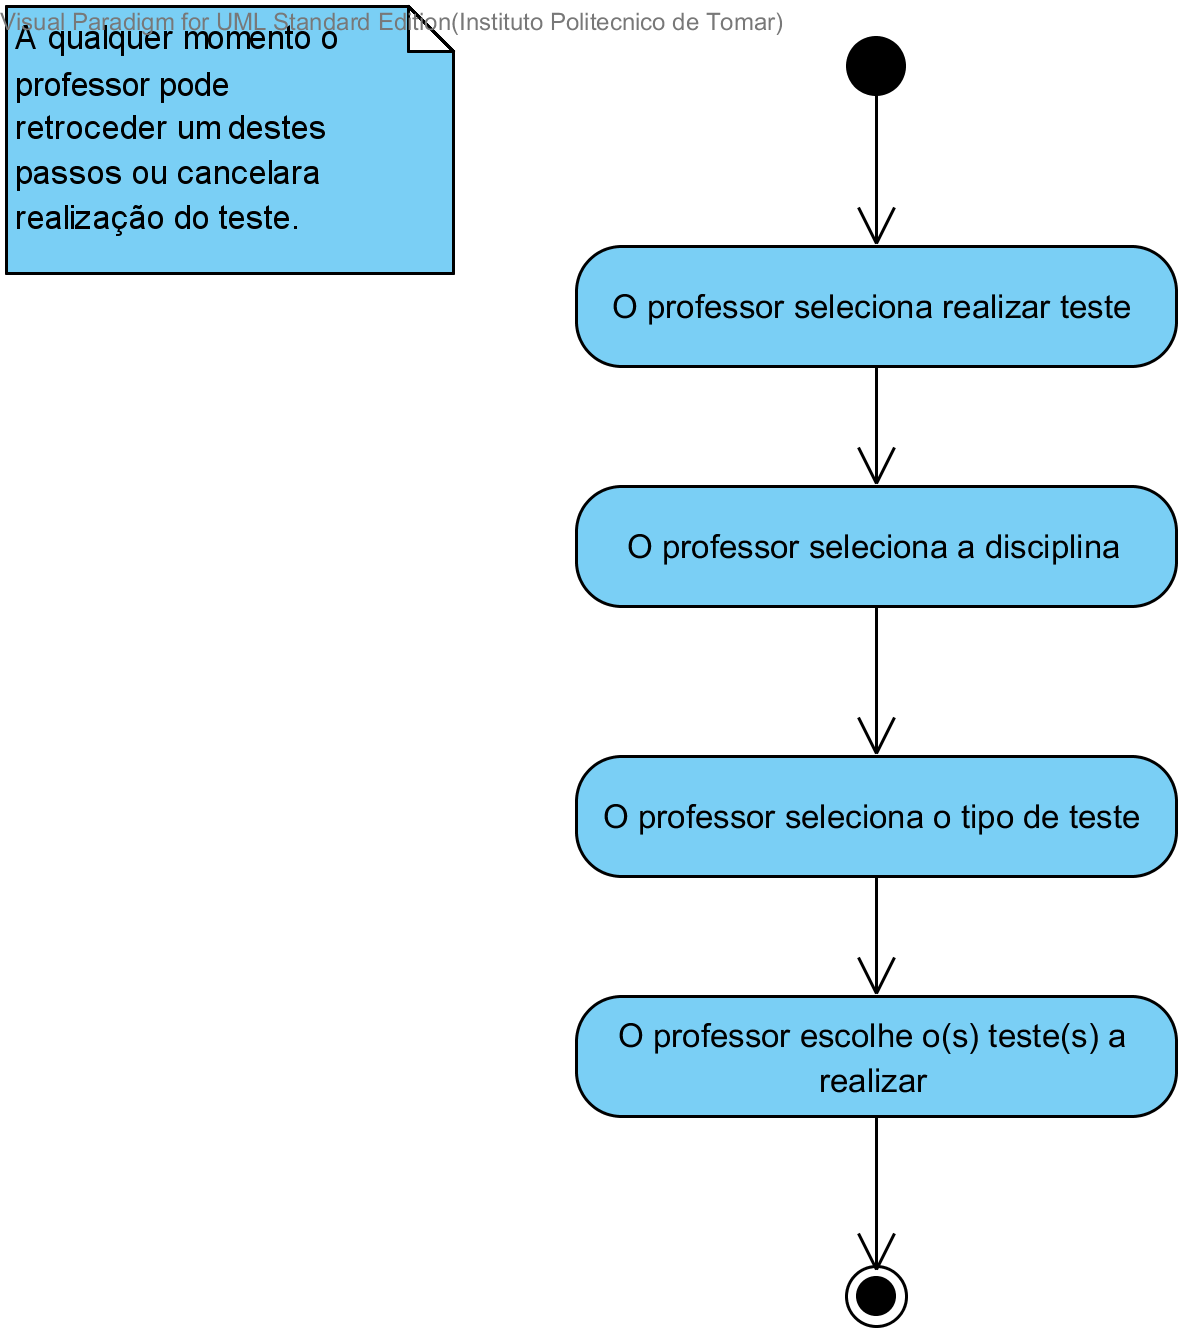
\includegraphics[width=0.8\linewidth]{./diagramasAnaliseSistemas/PrepararRealizacaodoTeste}
						\caption{Diagrama de actividades do C.U. preparar realização do teste.}
						\label{fig:PrepararRealizacaodoTeste}
					\end{figure}
					
					\newpage
					
					\begin{table}[h]
							\begin{tabular}{|p{2cm} p{10cm}|}
								\hline Nome: & Preparar Realização do Teste \\ 
								\hline Âmbito: & Letrinhas - APP \\ 
								\hline Finalidade: & Preparar a realização de um teste. \\ 
								\hline Atores: & Professor \\ 
							    \hline Pré-condições: & Deverão existir testes submetidos pelo  professor passíveis de realização.

								O professor deverá escolher a  Escola, escolher o professor, escolher a turma, seleccionar o aluno.
								 \\ 
							    \hline Sequência típica dos eventos: &  					
								O utilizador deve:
	    					\begin{enumerate}
							    \item	Seleccionar Realizar Teste;
								\item	Seleccionar Disciplina;
								\item	Seleccionar o tipo de teste;
								\item	Selecciona o teste a realizar.
						    \end{enumerate}  \\
								    \hline Sequências alternativas e extensões: & 
								    \begin{itemize}			    	
								  				    	\item O professor cancela a realização do teste.
								    \end{itemize}
								     \\ 
								    \hline Requisitos especiais: & Nenhum.\\ 
								    \hline Aspectos em aberto: & Nenhum. \\
													\hline 
							\end{tabular}
							\caption{Caso de utilização preparar realização de um teste.}
						\end{table} 
\newpage
					\subsubsection{Efectuar teste}
				
				
				\begin{figure}[h]
					\centering
					\includegraphics[width=0.8\linewidth]{./diagramasAnaliseSistemas/RealizarTeste}
					\caption{Diagrama de actividades do C.U. realizar teste}
					\label{fig:RealizarTeste}
					\end{figure}

					


				\newpage
				\begin {table}[h]
				\begin{tabular}{|p{2cm} p{10cm}|}
					\hline Nome: & CaU Efectuar teste \\ 
					\hline Âmbito: & Letrinhas - APP \\ 
					\hline Finalidade: & Correcção do teste. \\ 
					\hline Atores: & Aluno \\ 
				    \hline Pré-condições: & Deverão existir testes submetidos pelo  professor passíveis de realização.
					O professor deverá ter preparado a realização do teste. \\ 
				    \hline Sequência típica dos eventos: &  					
					O utilizador deve:
				    \begin{enumerate}
				    	\item	Efectuar a avaliação consoante o tipo de teste;
						\item	Submeter este para avaliação.
				    \end{enumerate} \\ 
  				    \hline Sequências alternativas e extensões: & 
  				    \begin{enumerate}			    	
  				    	\item[1a.] Se disponíveis poderá ouvir demonstrações;
						\item[2b.] O utilizador não submete a avaliação, cancelando a realização do teste.

  				    \end{enumerate}
  				     \\ 
  				    \hline Requisitos especiais: & Nenhum.\\ 
  				    \hline Aspectos em aberto: & Existem vários tipos de teste, cada um com algumas especificidades, estas não são descritas nesta tabela.  \\
					\hline 
				\end{tabular}
				\caption{Caso de utilização efectuar teste.}
			\end{table} 
			
		\newpage				
			\subsubsection{Efectuar Auto-avaliação}
						
				\begin{figure}[h]
\centering
\includegraphics[width=0.8\linewidth]{./diagramasAnaliseSistemas/EfectuarAutoAvaliacao}
\caption{Diagrama de actividade do CaU efectuar Auto-avaliação}
\label{fig:EfectuarAutoAvaliacao}
\end{figure}

		
							
		
		
						\newpage
						\begin {table}[h]
						\begin{tabular}{|p{2cm} p{10cm}|}
							\hline Nome: & CaU Efectuar Auto-avaliação \\ 
							\hline Âmbito: & Letrinhas - APP \\ 
							\hline Finalidade: & O ctor aluno poderá consultar testes previamente realizados por si, podendo desta forma avaliar o seu progresso.  \\ 
							\hline Atores: & Aluno \\ 
						    \hline Pré-condições: & DDeverão existir testes realizados pelo aluno já submetidos. \\ 
						    \hline Sequência típica dos eventos: &  					
							O utilizador deve:
						    \begin{enumerate}
						    	\item	Escolher quais os testes que pretende rever.
								\item	O utilizador carrega no botão de finalizar quando estiver satisfeito, avançando para outro teste.

						    \end{enumerate} \\ 
		  				    \hline Sequências alternativas e extensões: & 
		  				    \begin{enumerate}			    	
		  				    	\item[1a.] Se disponíveis poderá ouvir demonstrações, comparando com as suas submissões;
								\item[1b.] O utilizador não selecciona nenhum teste e aborta a operação.
								\item[2a.] O utilizador não seleccionou mais testes, finalizando assim a sequencia típica de eventos.

		
		  				    \end{enumerate}
		  				     \\ 
		  				    \hline Requisitos especiais: & Nenhum.\\ 
		  				    \hline Aspectos em aberto: & Existem vários tipos de teste, cada um com algumas especificidades, estas não são descritas nesta tabela.  \\
							\hline 
						\end{tabular}
						\caption{Caso de utilização efectuar Auto-avaliação.}
					\end{table} 
	\newpage
	\subsection{Descrição dos Casos de Utilização - Sistema de Informação}
	
	\subsubsection{Criar Novo Teste}
							
	\begin{figure}[h]
\centering
\includegraphics[width=0.7\linewidth]{./diagramasAnaliseSistemas/BackOfficecriartestedeLeitura}
\caption{Diagrama de Actividades do CaU criar novo teste.(teste de leitura)}
\label{fig:BackOfficecriartestedeLeitura}
\end{figure}

\begin{figure}[h]
\centering
\includegraphics[width=0.7\linewidth]{./diagramasAnaliseSistemas/testemultimedia}
\caption{Diagrama de Actividades do CaU criar novo teste.(teste de multimedia)}
\label{fig:testemultimedia}
\end{figure}



								
			
			
							\newpage
							\begin {table}[h]
							\begin{tabular}{|p{2cm} p{10cm}|}
								\hline Nome: & CaU Criar novo teste \\ 
								\hline Âmbito: & Letrinhas - SI \\ 
								\hline Finalidade: & Os atores envolvidos poderão criar testes, submetendo-os posteriormente para a Aplicação.  \\ 
								\hline Atores: & Professor, Administrador \\ 
							    \hline Pré-condições: & O utilizador deverá estar autenticado.\\ 
							    \hline Sequência típica dos eventos: &  					
								O utilizador deve:
							    \begin{enumerate}
							    	\item	Seleccionar o tipo de teste que pretende submeter para avaliação;
									\item	Preencher os devidos campos;
									\item	Submeter este.

	
							    \end{enumerate} \\ 
			  				    \hline Sequências alternativas e extensões: & 
			  				    \begin{enumerate}			    	
			  				    	\item[2a.] Consoante o tipo de teste o utilizador deverá submeter conteúdo multimédia.
									\item[3a.] O utilizador não submete o teste, cancelando a criação teste.

	
			
			  				    \end{enumerate}
			  				     \\ 
			  				    \hline Requisitos especiais: & Nenhum.\\ 
			  				    \hline Aspectos em aberto: & Existem vários tipos de teste, cada um com algumas especificidades, estas não são descritas nesta tabela.  \\
								\hline 
							\end{tabular}
							\caption{Caso de utilização efectuar criar novo teste.}
						\end{table} 
\newpage	
	\subsubsection{Criar registo de professor}
			\begin {table}[h]
									\begin{tabular}{|p{2cm} p{10cm}|}
										\hline Nome: & CaU Criar registo de professor \\ 
										\hline Âmbito: & Letrinhas - SI \\ 
										\hline Finalidade: & Os actores envolvidos poderão, adicionar professores.  \\ 
										\hline Atores: & Administrador \\ 
									    \hline Pré-condições: & O administrador deverá estar autenticado.\\ 
									    \hline Sequência típica dos eventos: &  					
										O utilizador deve:
									    \begin{enumerate}
									    \item	Seleccionar “Adicionar Professor”;
										\item	Preencher os devidos  campos (nome, email, telef, username, pin, escola  e fotografia);
										\item	Pressionar adicionar.

		
			
									    \end{enumerate} \\ 
					  				    \hline Sequências alternativas e extensões: & 
					  				    \begin{enumerate}			    	
					  				   \item[ 3a.] O utilizador não submete o professor, cancelando a inserção deste no sistema.
		
			
					
					  				    \end{enumerate}
					  				     \\ 
					  				    \hline Requisitos especiais: & Nenhum.\\ 
					  				    \hline Aspectos em aberto: & Nenhum  \\
										\hline 
									\end{tabular}
									\caption{Caso de utilização efectuar criar registo de professor}
								\end{table} 
	
	
	

\newpage
	\subsubsection{Criar registo de aluno}
			\begin {table}[h]
									\begin{tabular}{|p{2cm} p{10cm}|}
										\hline Nome: & CaU Criar registo de aluno\\ 
										\hline Âmbito: & Letrinhas - SI \\ 
										\hline Finalidade: & Os actores envolvidos poderão, adicionar alunos.  \\ 
										\hline Atores: & Administrador \\ 
									    \hline Pré-condições: & O administrador deverá estar autenticado.\\ 
									    \hline Sequência típica dos eventos: &  					
										O utilizador deve:
									    \begin{enumerate}
									    \item	Seleccionar “Adicionar Aluno”;
										\item	Preencher os devidos  campos (nome, escola, turma e fotografia);
										\item	Pressionar adicionar.


		
			
									    \end{enumerate} \\ 
					  				    \hline Sequências alternativas e extensões: & 
					  				    \begin{enumerate}			    	
					  				  \item[3a.] O utilizador não submete o aluno, cancelando a inserção deste no sistema.
		
			
					
					  				    \end{enumerate}
					  				     \\ 
					  				    \hline Requisitos especiais: & Nenhum.\\ 
					  				    \hline Aspectos em aberto: & Nenhum  \\
										\hline 
									\end{tabular}
									\caption{Caso de utilização efectuar criar registo de aluno}
								\end{table} 
	
	
	

\newpage

	\subsubsection{Criar escola}
			\begin {table}[h]
									\begin{tabular}{|p{2cm} p{10cm}|}
										\hline Nome: & CaU Criar escola\\ 
										\hline Âmbito: & Letrinhas - SI \\ 
										\hline Finalidade: & Os actores envolvidos poderão, inserir escolas no sistema.\\ 
										\hline Atores: & Administrador \\ 
									    \hline Pré-condições: & O administrador deverá estar autenticado.\\ 
									    \hline Sequência típica dos eventos: &  					
										O utilizador deve:
									    \begin{enumerate}
									    \item	Seleccionar “Adicionar Escola”;
										\item	Preencher os devidos  campos (nome, morada, fotografia);
										\item	Pressionar adicionar.



		
			
									    \end{enumerate} \\ 
					  				    \hline Sequências alternativas e extensões: & 
					  				    \begin{enumerate}			    	
					  				  \item[3a.] O utilizador não submete a escola, cancelando a inserção desta no sistema.
		
			
					
					  				    \end{enumerate}
					  				     \\ 
					  				    \hline Requisitos especiais: & Nenhum.\\ 
					  				    \hline Aspectos em aberto: & Nenhum  \\
										\hline 
									\end{tabular}
									\caption{Caso de utilização efectuar criar escola}
								\end{table} 
			
		
		\newpage
		
		\section{Modelo de dados persistente}
		
		\subsection{Modelo de dados persistente - Sistema de Informação}
		
		
		
		\begin{figure}[h]
			\centering
			\includegraphics[width=1.2\linewidth]{./diagramasAnaliseSistemas/modeloDeDadosPersistente}
			\caption{Modelo de dados Persistente.}
			\label{fig:modeloDeDadosPersistente}
		\end{figure}

		\newpage

		\section{Protótipo exploratório}
		
		\subsection{APP}
		
		\begin{figure}[h]
\centering
\includegraphics[width=1\linewidth]{./diagramasAnaliseSistemas/prototipoExploratorio/app/1}
\caption{Vista inicial.}
\label{fig:1}
\end{figure}

\begin{figure}[h]
\centering
\includegraphics[width=1\linewidth]{./diagramasAnaliseSistemas/prototipoExploratorio/app/2png}
\caption{Escolha da escola.}
\label{fig:2png}
\end{figure}

\newpage

\begin{figure}[h]
\centering
\includegraphics[width=1\linewidth]{./diagramasAnaliseSistemas/prototipoExploratorio/app/3}
\caption{Escolha do professor.}
\label{fig:3}
\end{figure}

\begin{figure}[h]
\centering
\includegraphics[width=1\linewidth]{./diagramasAnaliseSistemas/prototipoExploratorio/app/4}
\caption{Escolha da turma.}
\label{fig:4}
\end{figure}

\newpage

\begin{figure}[h]
\centering
\includegraphics[width=1\linewidth]{./diagramasAnaliseSistemas/prototipoExploratorio/app/5}
\caption{Escolha do aluno.}
\label{fig:5}
\end{figure}

\begin{figure}[h]
\centering
\includegraphics[width=1\linewidth]{./diagramasAnaliseSistemas/prototipoExploratorio/app/6}
\caption{Escolha do modo (realizar ou corrigir teste).}
\label{fig:6}
\end{figure}

\newpage

\subsection{Modo de realização de teste}

\begin{figure}[h]
\centering
\includegraphics[width=1\linewidth]{./diagramasAnaliseSistemas/prototipoExploratorio/app/14}
\caption{Escolha da disciplina.}
\label{fig:14}
\end{figure}

\begin{figure}[h]
\centering
\includegraphics[width=1\linewidth]{./diagramasAnaliseSistemas/prototipoExploratorio/app/8}
\caption{Escolha do tipo de teste.}
\label{fig:8}
\end{figure}
\newpage

\begin{figure}[h]
\centering
\includegraphics[width=1\linewidth]{./diagramasAnaliseSistemas/prototipoExploratorio/app/9}
\caption{Formulário de selecção dos testes a realizar}
\label{fig:9}
\end{figure}

\begin{figure}[h]
\centering
\includegraphics[width=1\linewidth]{./diagramasAnaliseSistemas/prototipoExploratorio/app/10}
\caption{Vista de um teste de leitura}
\label{fig:10}
\end{figure}

\newpage

\begin{figure}[h]
\centering
\includegraphics[width=1\linewidth]{./diagramasAnaliseSistemas/prototipoExploratorio/app/12}
\caption{Realizar Auto-avaliação}
\label{fig:12}
\end{figure}

\newpage

\subsection{Modo de Correcção de teste}


\begin{figure}[h]
\centering
\includegraphics[width=1\linewidth]{./diagramasAnaliseSistemas/prototipoExploratorio/app/17}
\caption{Ouvir a gravação submetida pelo aluno.}
\label{fig:17}
\end{figure}

\begin{figure}[h]
\centering
\includegraphics[width=1\linewidth]{./diagramasAnaliseSistemas/prototipoExploratorio/app/18}
\caption{Seleccionar das palavras erradas.}
\label{fig:18}
\end{figure}

\newpage

		\subsection{Sistema de Informação}
		
		\begin{figure}[h]
			\centering
			\includegraphics[width=0.8\linewidth]{./diagramasAnaliseSistemas/prototipoExploratorio/sistemaInformacao/1}
			\caption{Página inicial após autenticação.}
			\label{fig:1}
		\end{figure}
		
		\begin{figure}[h]
			\centering
			\includegraphics[width=0.8\linewidth]{./diagramasAnaliseSistemas/prototipoExploratorio/sistemaInformacao/2}
			\caption{Vista com lista de professores.}
			\label{fig:2}
		\end{figure}
\newpage
	\begin{figure}[h]
		\centering
		\includegraphics[width=0.8\linewidth]{./diagramasAnaliseSistemas/prototipoExploratorio/sistemaInformacao/3}
		\caption{Vista com lista de turmas.}
		\label{fig:3}
	\end{figure}

	\begin{figure}[h]
		\centering
		\includegraphics[width=0.8\linewidth]{./diagramasAnaliseSistemas/prototipoExploratorio/sistemaInformacao/4}
		\caption{Vista com lista de alunos.}
		\label{fig:4}
	\end{figure}
	
	\newpage
		\begin{figure}[h]
			\centering
			\includegraphics[width=0.8\linewidth]{./diagramasAnaliseSistemas/prototipoExploratorio/sistemaInformacao/6}
			\caption{Vista com listagem de testes.}
			\label{fig:5}
		\end{figure}
		
		\subsubsection{Criação de Testes}
		
		\begin{figure}[h]
				\centering
				\includegraphics[width=0.8\linewidth]{./diagramasAnaliseSistemas/prototipoExploratorio/sistemaInformacao/7}
				\caption{Vista com tipos de teste a inserir.}
				\label{fig:5}
			\end{figure}	
			
		\newpage

			\begin{figure}[h]
						\centering
						\includegraphics[width=0.8\linewidth]{./diagramasAnaliseSistemas/prototipoExploratorio/sistemaInformacao/8}
						\caption{Formulário de criação de teste multimédia (misto)}
						\label{fig:5}
					\end{figure}
	
		
				\begin{figure}[h]
					\centering
					\includegraphics[width=0.8\linewidth]{./diagramasAnaliseSistemas/prototipoExploratorio/sistemaInformacao/9}
					\caption{Formulário de criação de teste leitura}
					\label{fig:5}
				\end{figure}

		
		
		\section{Anexos}
		
		
					
\end{document}
 